\section{Durchführung}
\label{sec:Durchführung}
Der Veruch wird gemäß Abbildung\ref{fig:aufb} aufgebaut.
\begin{figure}[H]
  \centering
  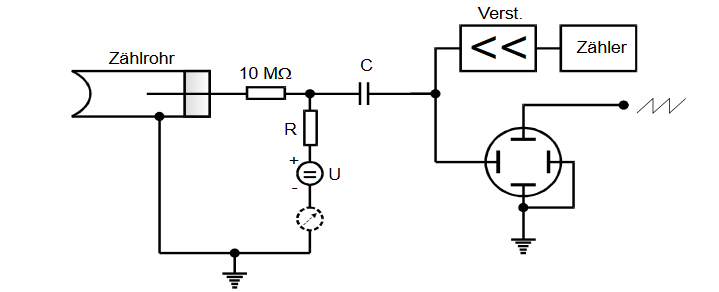
\includegraphics[scale=0.4]{content/Aufbau.png}
  \caption{Versuchsaufbau.}
  \label{fig:aufb}
\end{figure}

\subsection{Aufnahme der Charakteristik des Zählrohrs}
Der Strahlengang eines $\beta$-Strahlers wird auf das Zählrohr ausgerichtet.
Die Messung wird mit einer Anliegenden Spannung $U= 300 V$ begonnen.
Die Aktivität wird für $60$ Sekunden aufgenommen.
Zusätzlich wird mit einem empfindlichen Strommessgerät der Zählerstrom gemessen und über die Messzeit gemittelt.
Die Anliegende Spannung wird nach jeder so erfolgten Messung um $10 V$ erhöht bis eine Spannung von $700 V$ erreicht wird.
\subsection{Oszillographische Messung der Totzeit}
Das Zählrohr wird an ein Oszilloskop angeschlossen.
Die Zählrohrspannung wird auf $700$ Volt hochgestellt.
Aus dem so enstantendem Bild wird die Totzeit und die Erholungszeit abgelesen.
\subsection{Bestimmung der Totzeit mit der Zwei-Quellen-Methode}
Die Zählrohrspannung wird auf $500$ Volt geschaltet.
Die Aktivität des ausgerichteten Strahlers wird für $60$ Sekunden gemessen.
Ein zweiter, schwächerer, $\beta$-Strahler wird auf  das Zählrohr ausgerichtet.
Erneut wird die Aktivität für $60$ Sekunden gemessen.
Der erste $\beta$-Strahler wird entfernt und die Aktivität des zweiten Strahlers wird nach gleichem Verfahren gemessen.
